\chapter{Fault  analysis}
\textit{In this chapter, probable faults in the system are examined using a Failure Mode and Effects Analysis (FMEA). Next, in order to find how probable a fault will happen and the effect of it, the severity and occurrance (SO) of faults is analyzed. It was decided that the fault analysis will be carry out only for the actuators (magnetorquers and momentum wheels).}

A fault in a system can be seen as a sudden shift in the system functionality, nevertheless, it might not mean a total shutdown of the system. One way to see it is as a disturbance in the system, that might cause performance loss or serious deterioration to the system. On the other hand, a failure can be understood as a total shutdown of the system component. 

In \figref{fig:1} a fault tolerant system is described, which contains an autonomous supervisor that has the ability to switch between various controllers taking into account the type of fault that a component has. The spacecraft block illustrated in the picture is composed of a plant, actuators and sensors and is monitored by the fault detection and isolation (FDI) system, which include detectors that will feed informations to the supervisor in the eventuality of a fault. Based on the information received, the supervisor will establish if a fault occurred or not and in case of a fault the effectors will handle it. Figure \ref{fig:2} shows the procedure of how faults are handled with varius methods.

\begin{table}[H]
	\begin{minipage}[b]{0.49\linewidth}
		\centering
		\begin{figure}[H]
			\centering
			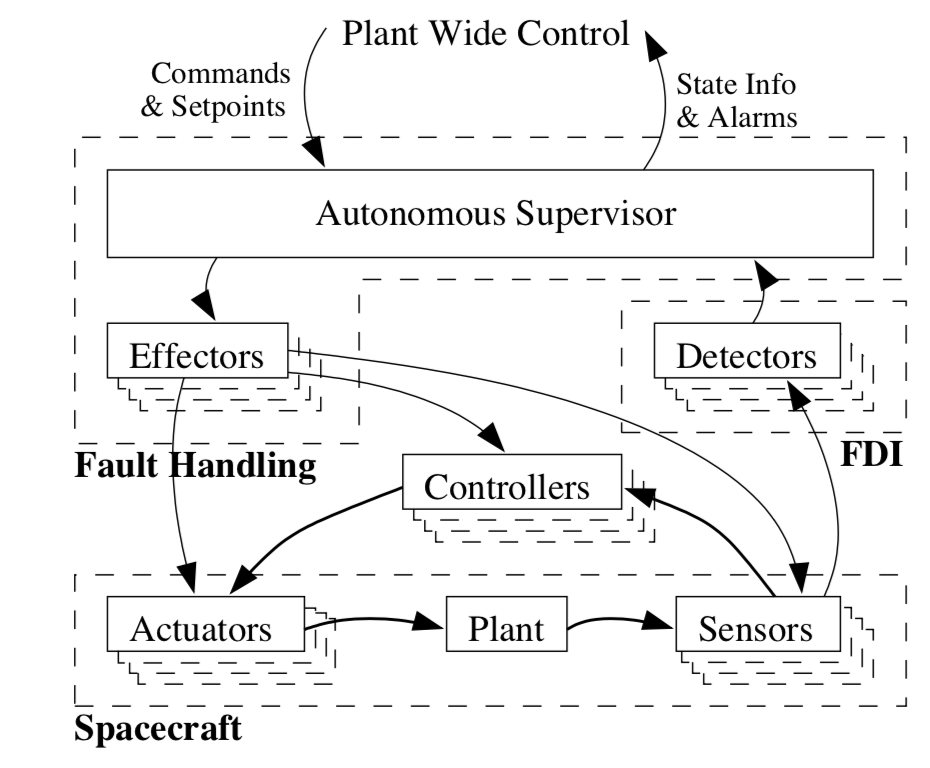
\includegraphics[width=1\linewidth]{figures/FTC}
			\caption{Fault tolerant system architecture [ref jesper article}
			\label{fig:1}
		\end{figure}
	\end{minipage}\hfill
	\begin{minipage}[b]{0.49\linewidth}
		\centering
		\begin{figure}[H]
			\centering
			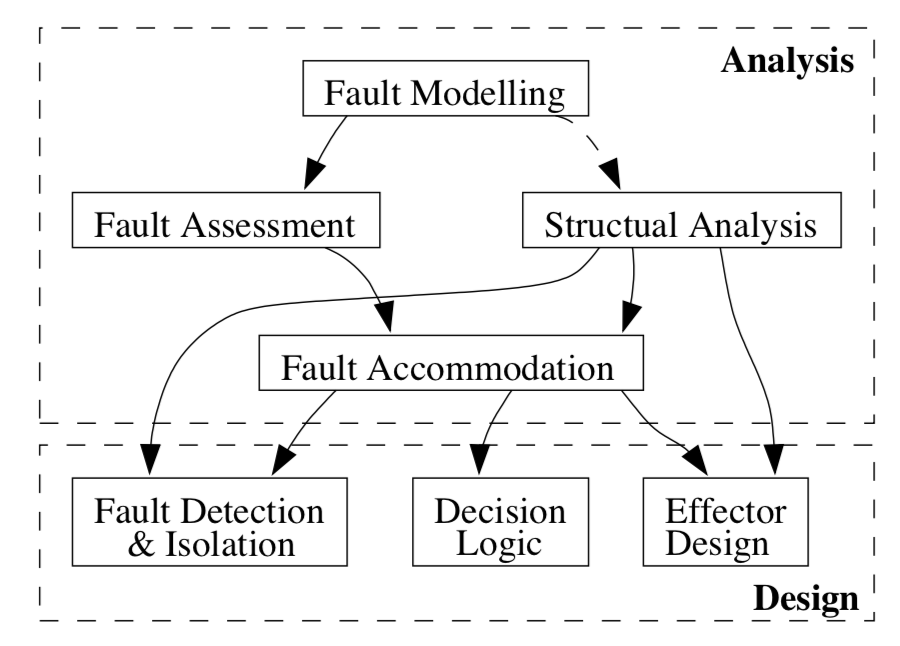
\includegraphics[width=1\linewidth]{figures/FTC_2}
			\caption{ }
			\label{fig:2}
		\end{figure}
	\end{minipage}
\end{table}

\subsection{Failure Mode and Effects Analysis}
A FMEA analysis which is a bottom-up analysis method is performed for the components of the satellite. The main goal of FMEA is to identify possible faults and their effects on components. In order to evaluate how faults are propagated through the system, a FMEA scheme is constructed.
Another aspect of FMEA analysis is that, the severity of a fault can be determined, which will offer the opportunity to prioritize the faults by severity and in this way focus on the important faults.

In order to control the attitude of the satellite, two types of actuators are used: magnetorquers and momentum wheels. Potential faults are gather into a table which describes the effect and cause, while the satellite is orbiting.
\subsubsection{Magnetorquers}

\begin{table}[H]
	\centering
	\label{my-label}
	\begin{tabular}{|l|l|l|}
		\hline
		\multicolumn{3}{|c|}{\textit{\textbf{Magnetorquers}}}                                          \\ \hline
		\multicolumn{3}{|c|}{Produces a magnetic field that interacts with Earth's magnetic field}                     \\ \hline
		\textbf{Reference} & \textbf{Failure Effect} & \textbf{Failure Cause}                          \\ \hline
		$MT_1$                 & Low magnetic field  & \begin{tabular}[c]{@{}l@{}}- Broken wire or bad soldering\\ - Component burned\end{tabular} \\ \hline
		$MT_2$                 & Maximum magnetic field power  & Short circuit to the power voltage   \\ \hline
		$MT_3$                 & Wrong direction of the magnetic field & \begin{tabular}[c]{@{}l@{}}- Misalignment of the magnetorquer\\ - Short circuit of some parts of the \\ torquer to the power voltage \end{tabular} \\ \hline
		$MT_4$                 & Wrong  power of the magnetic field                 & Floating supplay voltage                                            \\ \hline
	\end{tabular}
	\caption{Potential faults in the magnetorquers}
\end{table}

\subsubsection{Momentum wheels}

\begin{table}[H]
	\centering
	\label{my-label}
	\begin{tabular}{|l|l|l|}
		\hline
		\multicolumn{3}{|c|}{\textit{\textbf{Momentum wheels}}}                                          \\ \hline
		\multicolumn{3}{|c|}{Produces a torque about the satellite COM in order to rotate it }                     \\ \hline
		\textbf{Reference} & \textbf{Failure Effect} & \textbf{Failure Cause}                          \\ \hline
		$MW_1$                & Faulty orientation/alter the angular velocity & \begin{tabular}[c]{@{}l@{}} Shifting of the flywheel \\throughout launch or transport \\   \end{tabular} \\ \hline
		$MW_2$                & Unable to control the rotation   & A difference in the power voltage  \\ \hline
		$MW_3$                & No torque received& \begin{tabular}[c]{@{}l@{}} Short circuit to the ground\\  \end{tabular} \\ \hline
		$MW_4$                & Increased rotations of the flywheel  & Broken wire or bad soldering                                          \\ \hline
	\end{tabular}
	\caption{Potential faults in the momentum wheels}
\end{table}
\subsubsection{Severity and occurrence evaluation}
To investigate the faults that have the biggest rate of occurrence, the severity of the effects of failures and the probability of occurrence is determined based on the faults from FMEA. This procedure describes how to each fault receives a severity index (SO) and an occurrence index(OI). A table containing the serverity and occurrence for magnetorquers is shown as follows:
\begin{table}[H]
	\centering
	\label{11}
	\begin{tabular}{|l|l|l|l|}
		\hline
		\multicolumn{4}{|c|}{Magnetorquer}                                                                                         \\ \hline
		Reference & Severity & Occurrence                                          & SO Index                                      \\ \hline
		$MT_1$     & 7        & \begin{tabular}[c]{@{}l@{}}- 5\\ - 4\end{tabular} & \begin{tabular}[c]{@{}l@{}}- 35\\- 28\end{tabular} \\ \hline
		$MT_2$       & 10       & 3       & 30                \\ \hline
		$MT_3$       & 3        & \begin{tabular}[c]{@{}l@{}}- 2\\- 1\end{tabular} & \begin{tabular}[c]{@{}l@{}}- 6\\- 3\end{tabular} \\ \hline
		$MT_4$       & 4        & 6                   & 24                  \\ \hline
	\end{tabular}
\caption{SO for magnetorquer}
\end{table}
The same procedure is done for momentum wheels as follows:
\begin{table}[H]
	\centering
	\label{12}
	\begin{tabular}{|l|l|l|l|}
		\hline
		\multicolumn{4}{|c|}{Momentum wheels}                                                                                         \\ \hline
		Reference & Severity & Occurrence                                          & SO Index                                      \\ \hline
		$MW_1$      & 1        & \begin{tabular}[c]{@{}l@{}}7\\ \end{tabular} & \begin{tabular}[c]{@{}l@{}}7\\ \end{tabular} \\ \hline
		$MW_2$        & 1        & 4             & 4                                         \\ \hline
		$MW_3$        & 2        & \begin{tabular}[c]{@{}l@{}}3\\\end{tabular} & \begin{tabular}[c]{@{}l@{}}8\\ \end{tabular} \\ \hline
		$MW_4$        & 4        & 2     & 8               \\ \hline
	\end{tabular}
	\caption{SO for momentum wheels}
\end{table}

The severity index is computed using the following formula:
\begin{flalign}
	SO_{index} = severity \cdot occurrence
	\label{eq:ec1}
\end{flalign} 

\subsubsection{Fault propagation analysis}
In order to observe how faults are propagated through the system and the effect of these faults, a FMEA scheme is constructed. Further computation will be on the appendix.
\subsection{Fault detection and isolation}
